%!TEX program=xelatex
\documentclass[a4paper]{article}
\usepackage{ctex}
\usepackage{geometry}
\usepackage{graphicx}
\usepackage{float}

\geometry{left=3.0cm,right=3.0cm,top=3.5cm,bottom=3.5cm}

\title{与非门电路的测试}
\author{2017011341, 陈旭}
\date{2019 年 3 月}

\begin{document}

\maketitle

\section{实验目的}

    \begin{itemize}
        \item 测量 CMOS 与非门 CD4011、TTL 与非门 74LS00 的平均延迟时间和电压传输特性(只需测量传输特性曲线);
        \item 加深对与非门基本特性和主要参数的理解,掌握主要参数的测试方法。
    \end{itemize}

\section{实验原理}

    \subsection{CMOS 与非门平均延迟时间的测量}
    
        \begin{figure}[H]
            \centering
            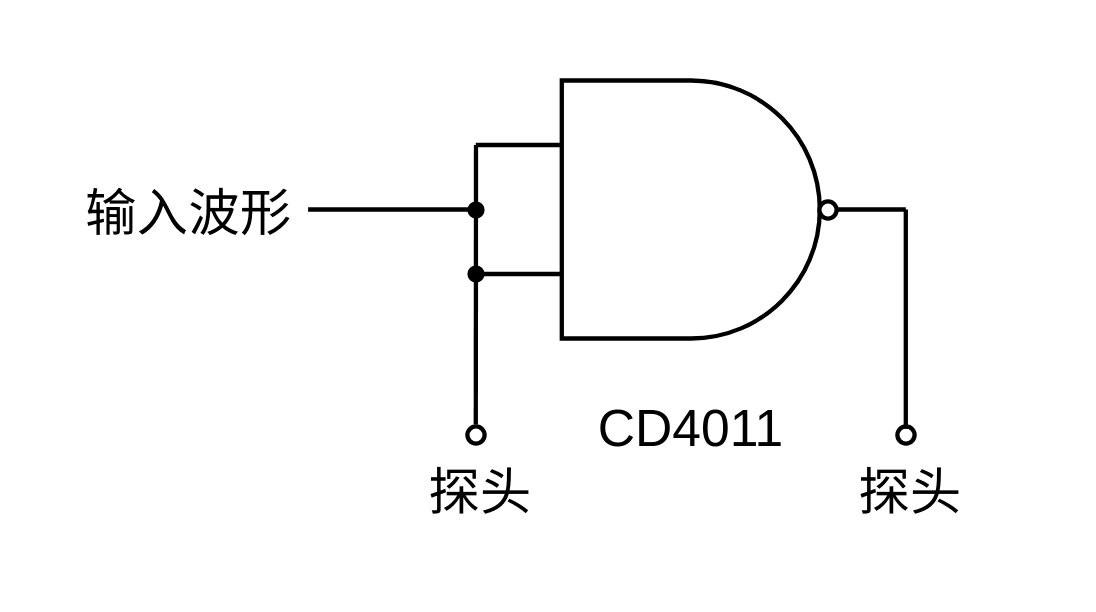
\includegraphics[width=0.7\linewidth]{figures/f1}
            \caption{测量 CMOS 与非门 CD4011 平均延迟时间原理图}
        \end{figure}

		\par 原理图如图 1 所示,测量边沿延迟时间 $t_{pHL}$ 表示探头 1 处于上升沿,探头 2 处于下降沿,$t_{pLH}$ 反之,则 $t_{pd}=(t_{pHL}+t_{pLH})/2$。

    \subsection{TTL 与非门平均延迟时间的测量}

        \begin{figure}[H]
            \centering
            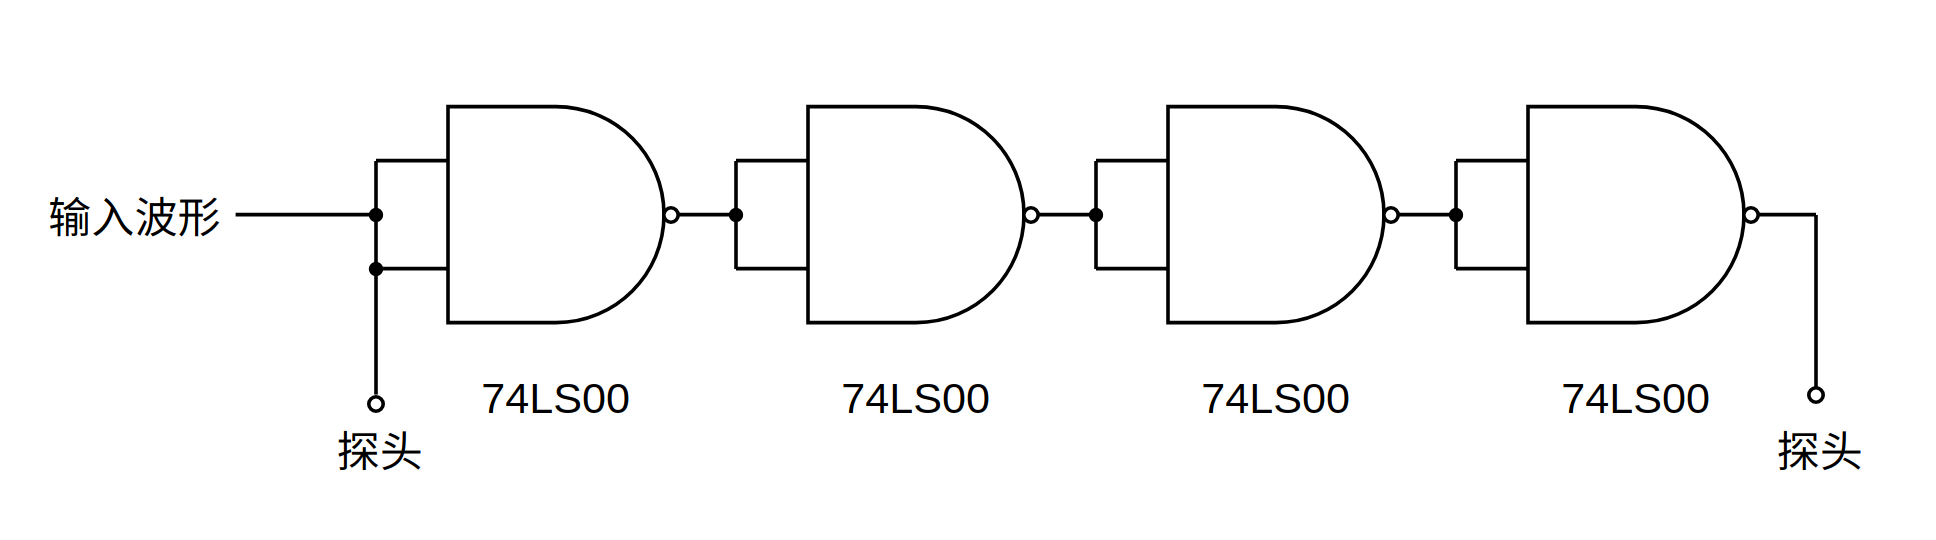
\includegraphics[width=0.7\linewidth]{figures/f2}
            \caption{测量 TTL 与非门 74LS00 平均延迟时间原理图}
        \end{figure}

        \par 原理图如图 2 所示,由于 TTL 与非门 74LS00 的平均延迟时间较短,所以叠加四级逻辑门后取平均。故 $t_{pd}=(t_{pHL}+t_{pLH})/8$。

    \subsection{电压传输特性的测量}

        \begin{figure}[H]
            \centering
            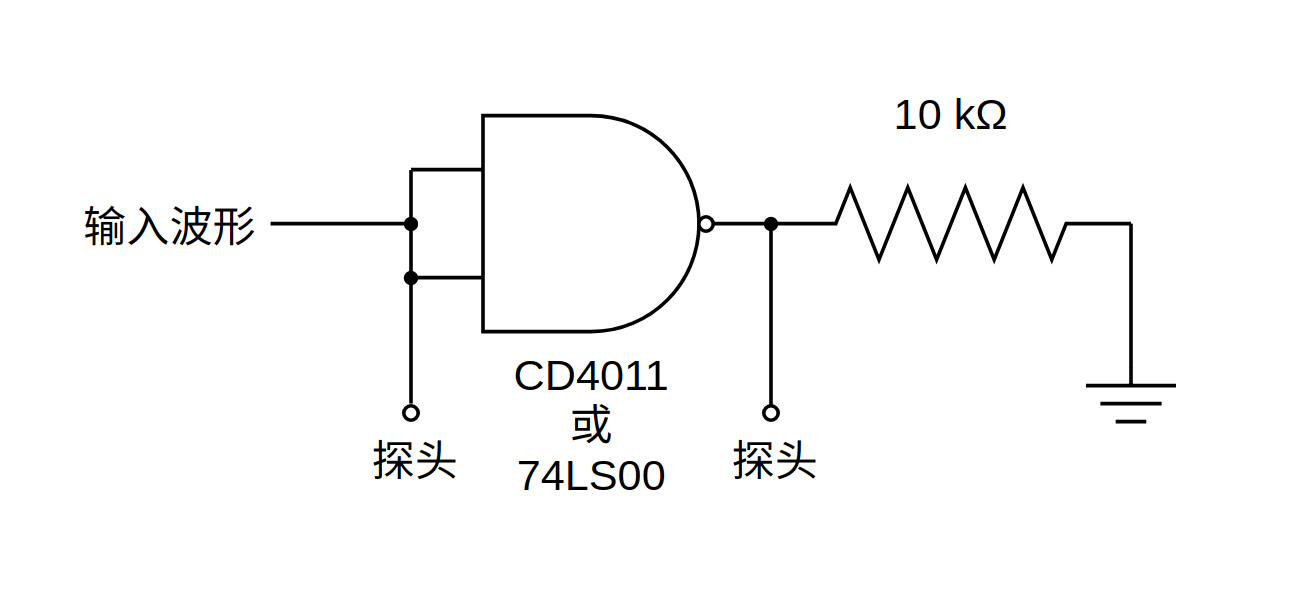
\includegraphics[width=0.7\linewidth]{figures/f3}
            \caption{测量电压传输特性原理图}
        \end{figure}

		\par 测量两种与非门的方法相同,原理图如图 3 所示。

\section{实验步骤}

    \subsection{测量平均延迟时间}

        \begin{itemize}
            \item 正确连接电路;
            \item 调整探头的衰减常数与示波器的探头参数,探头衰减常数选用 “$\times 10$”;
            \item 用示波器生成指定频率的 TTL 方波;
            \item 使用示波器的测量功能进行测量,设置好探头对应的边沿,即可分别得到 $t_{pHL}$ 和 $t_{pLH}$;
            \item 通过公式计算出平均延迟时间。
        \end{itemize}

    \subsection{测量电压传输特性}

        \begin{itemize}
            \item 正确连接电路;
            \item 调整探头的衰减常数与示波器的探头参数,探头衰减常数选用 “$\times 1$”;
            \item 用示波器生成指定频率的三角波;
            \item 使用时基模式切换显示模式,得到电压特性曲线。
        \end{itemize}

\section{注意事项}

    \begin{itemize}
        \item 波形未调试好前不能将其接入芯片;
        \item 确保芯片引脚与插座正确连接;
        \item 检查芯片接电源和地;
        \item 插线及更换元件应先断电;
        \item 输入端不得悬空,不用时应确定电平;
        \item 电路工作不正常时,首先通过集成电路的管脚处测试芯片的电源和地引脚。
    \end{itemize}

\end{document}